\documentclass[border=6pt,tikz]{standalone}
\usepackage{tikz}
\usepackage{amsmath,amssymb}
\usetikzlibrary{arrows.meta,positioning,fit,backgrounds,calc,shapes.geometric,decorations.pathreplacing,patterns}
\definecolor{ink}{HTML}{1B2430}
\definecolor{muted}{HTML}{6B7785}
\definecolor{accent}{HTML}{2F6FB5}
\definecolor{accent2}{HTML}{C1611F}
\definecolor{good}{HTML}{2E7D5B}
\definecolor{soft}{HTML}{EDF2F7}
\definecolor{soft2}{HTML}{FBEDE2}
\definecolor{soft3}{HTML}{E6F0E9}
\tikzset{
  box/.style={draw=ink,line width=.7pt,rounded corners=2pt,fill=soft,inner sep=4pt,align=center,font=\sffamily\small},
  boxa/.style={box,fill=soft2},
  boxb/.style={box,fill=soft3},
  plain/.style={align=center,font=\sffamily\small,text=ink},
  tiny/.style={align=center,font=\sffamily\scriptsize,text=muted},
  ar/.style={-{Stealth[length=2.4mm]},draw=ink,line width=.7pt},
  arm/.style={-{Stealth[length=2.4mm]},draw=muted,line width=.6pt,dashed},
  nd/.style={circle,draw=ink,line width=.7pt,fill=white,minimum size=7mm,inner sep=0pt,font=\sffamily\scriptsize},
  ndf/.style={nd,fill=soft},
  ndt/.style={nd,fill=soft2},
}

\begin{document}
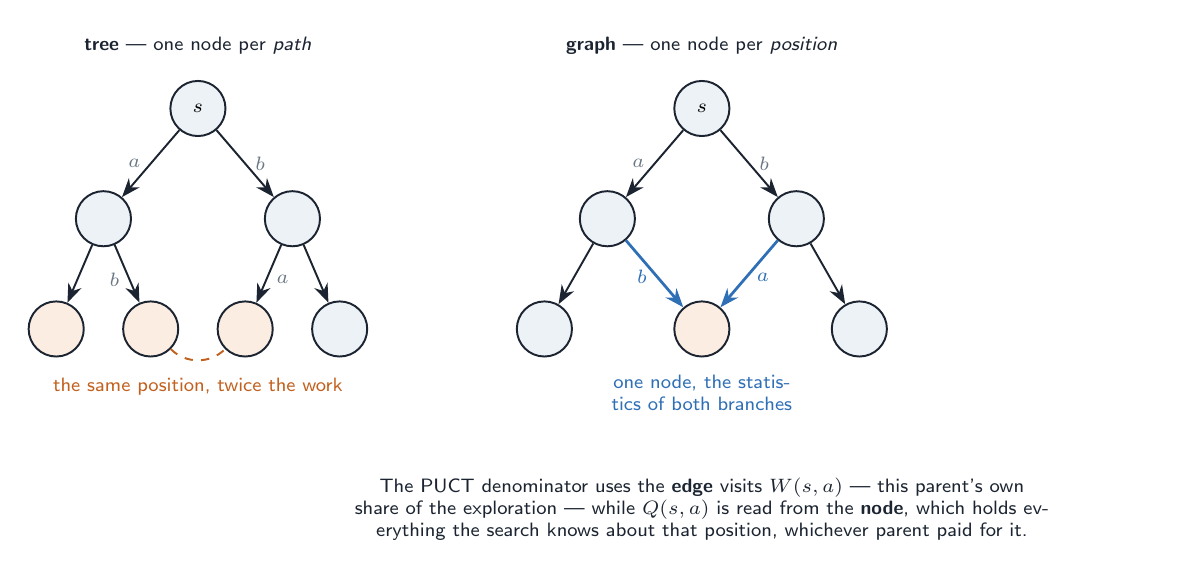
\begin{tikzpicture}[x=1mm,y=1mm]
  % ── tree ──
  \begin{scope}
    \node[tiny,text=ink] at (18,42) {\textbf{tree} --- one node per \emph{path}};
    \node[ndf] (r) at (18,34) {$s$};
    \node[ndf] (a) at (6,20) {}; \node[ndf] (b) at (30,20) {};
    \node[ndt] (c1) at (0,6) {}; \node[ndt] (c2) at (12,6) {}; \node[ndt] (c3) at (24,6) {}; \node[ndf] (c4) at (36,6) {};
    \draw[ar] (r)--node[tiny,left]{$a$}(a); \draw[ar] (r)--node[tiny,right]{$b$}(b);
    \draw[ar] (a)--(c1); \draw[ar] (a)--node[tiny,left,pos=.6]{$b$}(c2);
    \draw[ar] (b)--node[tiny,right,pos=.6]{$a$}(c3); \draw[ar] (b)--(c4);
    \draw[draw=accent2,dashed,line width=.7pt] (c2) to[bend right=45] node[tiny,below,text=accent2,text width=38mm,yshift=-1mm] {the same position, twice the work} (c3);
  \end{scope}
  % ── dag ──
  \begin{scope}[shift={(64,0)}]
    \node[tiny,text=ink] at (18,42) {\textbf{graph} --- one node per \emph{position}};
    \node[ndf] (R) at (18,34) {$s$};
    \node[ndf] (A) at (6,20) {}; \node[ndf] (B) at (30,20) {};
    \node[ndt] (C) at (18,6) {}; \node[ndf] (D) at (38,6) {}; \node[ndf] (E) at (-2,6) {};
    \draw[ar] (R)--node[tiny,left]{$a$}(A); \draw[ar] (R)--node[tiny,right]{$b$}(B);
    \draw[ar] (A)--(E);
    \draw[ar,draw=accent,line width=1pt] (A)--node[tiny,left,pos=.55,text=accent]{$b$}(C);
    \draw[ar,draw=accent,line width=1pt] (B)--node[tiny,right,pos=.55,text=accent]{$a$}(C);
    \draw[ar] (B)--(D);
    \node[tiny,below=1mm of C,text=accent,text width=44mm] {one node, the statistics of both branches};
  \end{scope}
  \node[tiny,below=14mm of C,text width=115mm,text=ink] {The PUCT denominator uses the \textbf{edge} visits $W(s,a)$ --- this parent's own share of
    the exploration --- while $Q(s,a)$ is read from the \textbf{node}, which holds everything the search knows about that
    position, whichever parent paid for it.};
\end{tikzpicture}
\end{document}
